\section{问题三的模型建立与求解}

无线电源搜索可根据观测条件调整不同阶段的行动策略\textsuperscript{\cite{ref4}}。前两问以单个干扰源为对象，根据示向度缩小位置范围，并比较不同检测位置的定位效果。第三问中，机器狗既要处理已经发现的源，又要继续排查尚未发现的源，两类任务共用同一条行进路线。一次新的观测不仅改变定位区域，也可能增加清除任务或减少后续巡测范围。因此，本问建立``基于覆盖约束的搜索-清除联合规划模型''，在维持排查完整性的前提下，设计机器狗的寻路策略。

\subsection{模型建立}

\subsubsection{状态与行动}

源搜索可通过观测更新信念状态并据此选择后续行动\textsuperscript{\cite{ref7}}。我们定义离散指标 \(t=0,1,\ldots\) 表示第 \(t\) 个行动开始前的决策步，该指标以行动序号计量。频道集合记为 \(\mathcal C=\{1,\ldots,20\}\)，目标可能出现的区域为：
\[
\Omega=\{g\in\mathbb R^2:\|g\|_2\le1800\}
\]

在决策步 \(t\)，记机器狗当前位置为 \(p_t\)，测向机当前频道为 \(\kappa_t\)。记 \(\mathcal D_t\) 为已发现但尚未清除的频道集合，\(\mathcal N_t\) 为尚未发现干扰源的频道集合。当频道被成功清除时，不再属于上述两个集合。

对 \(c\in\mathcal D_t\)，源位置 \(g\) 与该源在频道 \(c\) 的有效接收半径 \(R\) 构成一个组合 \((g,R)\)。能够同时解释该频道截至当前全部检测结果的组合构成集合 \(\mathcal X_{c,t}\)：
\[
\mathcal X_{c,t}\subseteq\Omega\times[1000,1500]
\]

其中，\(g\) 为源的可能位置，\(R\) 为该源在频道 \(c\) 的有效接收半径，同一个源在历次检测中对应同一个 \(R\)。\(F_{c,t}=\operatorname{proj}_g\mathcal X_{c,t}\) 为这些组合对应的定位区域，由每个组合中取出位置分量 \(g\) 得到。对 \(c\in\mathcal N_t\)，以 \(H^-_{c,t}\) 记录截至当前在频道 \(c\) 上测得无信号的全部检测点坐标，该频道尚未排除的目标区域为：
\[
U_{c,t}
=
\Omega\setminus
\bigcup_{h\in H^-_{c,t}}\overline B(h,1000)
\]

其中，\(h\) 为频道 \(c\) 的无信号检测点坐标，\(\overline B(h,1000)\) 为以 \(h\) 为圆心、半径 1000 米的闭圆盘。全向源的接收半径不小于 1000 米，由此在 \(h\) 处测得无信号即排除以 \(h\) 为圆心、半径 1000 米的圆盘。借鉴马尔可夫决策过程的序贯决策思想，定义信息状态为：
\[
S_t=
\left(
p_t,\kappa_t,\mathcal D_t,\mathcal N_t,
\{\mathcal X_{c,t}:c\in\mathcal D_t\},
\{H^-_{c,t},U_{c,t}:c\in\mathcal N_t\}
\right)
\tag{20}
\]

机器狗在状态 \(S_t\) 下选择行动：
\[
a_t=(o_t,q_t,c_t)=\pi(S_t)
\tag{21}
\]

其中，\(o_t\in\{\text{检测},\text{清除}\}\) 为本次行动类型，\(q_t\) 为本次行动的位置，\(c_t\) 为目标频道，\(\pi\) 为根据当前状态选择下一行动的策略。

\subsubsection{状态转移}

记 \(y_t\) 为行动 \(a_t\) 得到的反馈，下一状态为：
\[
S_{t+1}=\Phi(S_t,a_t,y_t),
\qquad
p_{t+1}=q_t,
\qquad
\kappa_{t+1}=
\begin{cases}
c_t,&o_t=\text{检测},\\
\kappa_t,&o_t=\text{清除}
\end{cases}
\tag{22}
\]

除下述与频道 \(c_t\) 有关的状态外，其余频道的信息保持不变。状态转移算子 \(\Phi\) 按行动类型分为检测与清除两部分。

\paragraph{检测行动}

检测反馈可能为近距离、示向度或无信号。根据频道此前是否已被发现，模型分别进行如下更新。

（1）检测已发现频道。 当 \(c_t\in\mathcal D_t\) 时，该频道此前得到的全部可能组合为 \(\mathcal X_{c_t,t}\)。三类反馈分别给出：
\[
\mathcal X_{c_t,t+1}=
\begin{cases}
\{(g,R)\in\mathcal X_{c_t,t}:\|g-q_t\|_2\le5\},
&y_t=\text{近距离},\\[1mm]
\{(g,R)\in\mathcal X_{c_t,t}:g\in W(q_t,\beta),\ 5<\|g-q_t\|_2\le R\},
&y_t=\text{示向度 }\beta,\\[1mm]
\{(g,R)\in\mathcal X_{c_t,t}:\|g-q_t\|_2>R\},
&y_t=\text{无信号}
\end{cases}
\tag{23a}
\]

更新后的定位区域为：
\[
F_{c_t,t+1}=\operatorname{proj}_g\mathcal X_{c_t,t+1}
\]

上述更新均在 \(\mathcal X_{c_t,t}\) 给出的组合中进行，因此更新后的组合仍能解释该频道此前的全部检测结果。

（2）检测未发现频道。 当 \(c_t\in\mathcal N_t\) 时，根据返回结果分为无信号与有信号两种情况。

\begin{enumerate}
\def\labelenumi{\arabic{enumi}.}
\tightlist
\item
  返回无信号。 该频道仍未被发现。由于全向源的接收半径不小于1000米，可排除检测点周围1000米范围：
\end{enumerate}
\[
H^-_{c_t,t+1}=H^-_{c_t,t}\cup\{q_t\},
   \qquad
   U_{c_t,t+1}=U_{c_t,t}\setminus\overline B(q_t,1000)
   \tag{23b}
\]

\begin{enumerate}
\def\labelenumi{\arabic{enumi}.}
\setcounter{enumi}{1}
\tightlist
\item
  返回信号。 该频道被发现。先根据此前的全部无信号记录构造：
\end{enumerate}
\[
\mathcal X^-_{c_t,t}
   =
   \{(g,R)\in\Omega\times[1000,1500]:
   \|g-h\|_2>R,\ \forall h\in H^-_{c_t,t}\}
\]

再根据本次信号类型更新：
\[
\mathcal X_{c_t,t+1}=
   \begin{cases}
   \{(g,R)\in\mathcal X^-_{c_t,t}:\|g-q_t\|_2\le5\},
   &y_t=\text{近距离},\\[1mm]
   \{(g,R)\in\mathcal X^-_{c_t,t}:g\in W(q_t,\beta),\ 5<\|g-q_t\|_2\le R\},
   &y_t=\text{示向度 }\beta
   \end{cases}
   \tag{23c}
\]

随后更新定位区域与频道集合为：
\[
F_{c_t,t+1}=\operatorname{proj}_g\mathcal X_{c_t,t+1},
   \qquad
   \mathcal D_{t+1}=\mathcal D_t\cup\{c_t\},
   \qquad
   \mathcal N_{t+1}=\mathcal N_t\setminus\{c_t\}
\]

\paragraph{清除行动}

清除行动仅针对 \(c_t\in\mathcal D_t\) 执行，并根据结果分为以下两种情况。

\begin{enumerate}
\def\labelenumi{\arabic{enumi}.}
\tightlist
\item
  清除成功。 该频道的干扰源已被处理，将其从待清除集合中删除：
\end{enumerate}
\[
\mathcal D_{t+1}=\mathcal D_t\setminus\{c_t\}
\]

\begin{enumerate}
\def\labelenumi{\arabic{enumi}.}
\setcounter{enumi}{1}
\tightlist
\item
  清除失败。 由失败反馈可知真实位置不在清除点周围20米内，因此更新：
\end{enumerate}
\[
\mathcal X_{c_t,t+1}
   =
   \{(g,R)\in\mathcal X_{c_t,t}:\|g-q_t\|_2>20\},
   \qquad
   F_{c_t,t+1}=\operatorname{proj}_g\mathcal X_{c_t,t+1}
   \tag{23d}
\]

\subsubsection{保证清除区域与候选行动}

对 \(c\in\mathcal D_t\)，定义保证清除区域：
\[
\mathcal G_{c,t}
=
\left\{q\in\mathbb R^2:
\sup_{g\in F_{c,t}}\|g-q\|_2\le20
\right\}
=
\bigcap_{g\in F_{c,t}}\overline B(g,20)
\tag{24}
\]

\(\mathcal G_{c,t}\) 中的任一点到全部可能真实位置的距离均不超过20米，因而能够保证清除成功。由最小包围圆的定义得：
\[
\mathcal G_{c,t}\ne\varnothing
\quad\Longleftrightarrow\quad
\rho(F_{c,t})\le20
\]

当 \(\mathcal G_{c,t}\ne\varnothing\) 时，选择距离当前位置最近的保证清除点：
\[
q_{c,t}^{\mathrm{clr}}
\in
\arg\min_{q\in\mathcal G_{c,t}}\|q-p_t\|_2,
\]

并构造清除候选行动集合：
\[
\mathcal A_t^{\mathrm{clr}}
=
\left\{
(\text{清除},q_{c,t}^{\mathrm{clr}},c):
c\in\mathcal D_t,
\mathcal G_{c,t}\ne\varnothing
\right\}
\tag{25}
\]

当 \(\mathcal G_{c,t}=\varnothing\) 时，当前信息不足以保证清除成功，故后续检测用于缩小 \(F_{c,t}\)。因此，\(\mathcal G_{c,t}\) 决定频道 \(c\) 在当前阶段生成``补充检测行动''还是``保证清除行动''，而 \(\mathcal A_t^{\mathrm{clr}}\) 将几何定位结果直接转化为后续路线中的可执行任务。

\subsubsection{完整排查与终止条件}

对每个 \(c\in\mathcal N_t\)，记 \(\mathcal P_{c,t}\) 为后续计划检测该频道的位置集合。由于未知干扰源的接收半径至少为1000米，为完整排查当前未排除区域，要求：
\[
U_{c,t}
\subseteq
\bigcup_{q\in\mathcal P_{c,t}}\overline B(q,1000),
\qquad c\in\mathcal N_t
\tag{26}
\]

当所有已发现源均已清除，且所有尚未发现频道的可能区域均已排空时，任务完成。策略 \(\pi\) 的终止步定义为：
\[
\tau_\pi
=
\inf\left\{
t:\mathcal D_t=\varnothing,
\quad
U_{c,t}=\varnothing,\ \forall c\in\mathcal N_t
\right\}
\tag{27}
\]

模型将``退出''并入终止条件，任务在满足式（27）时自然终止。由于每次行动均满足 \(p_{t+1}=q_t\)，因此，最终位置也将满足 \(p_{\tau_\pi}=q_{\tau_\pi-1}\)。

\subsubsection{时间代价与优化目标}

行动 \(a_t\) 的实际耗时为：
\[
\ell(S_t,a_t,y_t)
=
\frac{\|q_t-p_t\|_2}{5}
+
\begin{cases}
5+\mathbf 1_{\{c_t\ne\kappa_t\}},&o_t=\text{检测},\\[1mm]
5,&o_t=\text{清除且成功},\\[1mm]
3,&o_t=\text{清除且失败}
\end{cases}
\tag{28}
\]

其中，检测完成后测向机频道变为 \(c_t\)，清除操作不改变当前频道。策略 \(\pi\) 的完整任务时间为：
\[
T_{\mathrm{exit}}(\pi)
=
\sum_{t=0}^{\tau_\pi-1}\ell(S_t,a_t,y_t)
\tag{29}
\]

问题三的优化目标为：
\[
\min_{\pi\in\Pi_{\mathrm{adm}}}
\mathbb E\!\left[T_{\mathrm{exit}}(\pi)\right],
\tag{30}
\]

其中，\(\Pi_{\mathrm{adm}}\) 为满足状态转移式（22）---（23）、完整排查约束式（26）与终止条件式（27）的可行策略集合。式（27）保证全部干扰源最终被发现并清除，式（30）则在此前提下比较不同策略的平均完成时间。

\subsection{模型的滚动规划求解}

\subsubsection{模型特点与算法选择}

采用精确动态规划时，价值函数满足：
\[
V(S)
=
\min_{a\in\mathcal A(S)}
\mathbb E\!\left[
\ell(S,a,Y)+V\bigl(\Phi(S,a,Y)\bigr)
\mid S,a
\right],
\tag{31}
\]

其中，\(\mathcal A(S)\) 为当前状态下的可行行动集合。然而因为直接求解式（31）的计算量过大，所以我们借鉴模型预测控制的滚动优化思想，采用``基于条件场景评估的启发式滚动规划算法''：由式（26）保证排查的完整性，利用问题二的定位区域更新与选点方法处理已发现源，再通过有限候选路线与条件场景比较当前行动。每次只执行所选路线中的第一个行动，并根据反馈重新计算下一步。

\subsubsection{当前候选行动与条件场景}

在状态 \(S_t\) 下构造三类候选行动：

\begin{enumerate}
\def\labelenumi{\arabic{enumi}.}
\tightlist
\item
  对 \(c\in\mathcal N_t\)，根据式（26）生成未知频道检测行动，组成 \(\mathcal A_t^{\mathrm{scan}}\)；
\item
  对 \(c\in\mathcal D_t\) 且 \(\mathcal G_{c,t}=\varnothing\)，根据当前 \(F_{c,t}\) 与问题二的选点方法生成补充检测行动，组成 \(\mathcal A_t^{\mathrm{loc}}\)；
\item
  对 \(c\in\mathcal D_t\) 且 \(\mathcal G_{c,t}\ne\varnothing\)，按式（25）生成保证清除行动，组成 \(\mathcal A_t^{\mathrm{clr}}\)。
\end{enumerate}

由此得到：
\[
\mathcal A_t
=
\mathcal A_t^{\mathrm{scan}}
\cup\mathcal A_t^{\mathrm{loc}}
\cup\mathcal A_t^{\mathrm{clr}}
\]

仅比较当前已经生成的行动会忽略后续可能发现的新源。为估计这部分附加代价，我们根据未知频道的无信号历史构造条件场景。条件于频道 \(c\) 确实存在干扰源，候选位置 \(g\) 处允许的接收半径上界与相容权重为：
\[
R^{\max}_{c,t}(g)
=
\min\left\{
1500,
\min_{h\in H^-_{c,t}}\|g-h\|_2
\right\},
\qquad
w_{c,t}(g)
=
\left[R^{\max}_{c,t}(g)-1000\right]_+
\tag{32}
\]

当 \(H^-_{c,t}=\varnothing\) 时取 \(R^{\max}_{c,t}(g)=1500\)。按归一化后的 \(w_{c,t}(g)\) 抽取潜在位置，并结合10---16个源、频道互不重复的条件生成 \(B\) 个场景。

\subsubsection{候选路线评价}

由当前候选行动，我们构造若干从 \(p_t\) 出发的开放路线，记其集合为 \(\Sigma_t\)。对 \(\sigma\in\Sigma_t\)，记完成当前确定行动的代价为 \(C_t^{\mathrm{known}}(\sigma)\)；在场景 \(\omega\) 下，将可能新发现的源插入其首次可检测位置之后，产生的附加移动距离记为 \(\Delta L_t(\sigma,\omega)\)。

设频道 \(c\) 当前剩余的检测行动数为 \(k_{c,t}\)，场景 \(\omega\) 中实际存在源的未发现频道集合为 \(E(\omega)\)，频道 \(c\) 首次被发现前执行的检测行动数为 \(j_c(\sigma,\omega)\)，则未来频道检测次数近似为：
\[
N_t^{\mathrm{future}}(\sigma,\omega)
=
\sum_{c\in\mathcal N_t\setminus E(\omega)}k_{c,t}
+
\sum_{c\in E(\omega)}j_c(\sigma,\omega)
\]

候选路线的代理代价取为：
\[
\widetilde T_t(\sigma,\omega)
=
C_t^{\mathrm{known}}(\sigma)
+\frac{\Delta L_t(\sigma,\omega)}{5}
+6N_t^{\mathrm{future}}(\sigma,\omega)
\tag{33}
\]

其中，6秒近似一次检测与一次频道切换的代价，并选择：
\[
\sigma_t^*
\in
\arg\min_{\sigma\in\Sigma_t}
\frac1B\sum_{b=1}^{B}\widetilde T_t(\sigma,\omega_b)
\tag{34}
\]

滚动策略取所选路线的第一个行动，即：
\[
\pi_{\mathrm{roll}}(S_t)=\operatorname{First}(\sigma_t^*)
\]

图\ref{fig:q3-scenario-routes}以同一条件场景说明式（33）的代价估计。图中\(g\)为场景中假设存在的频道\(c\)干扰源，\(q_1,q_2\)为巡测点，\(A,B\)分别为补测与清除任务的执行位置。

\begin{figure}[H]
\centering
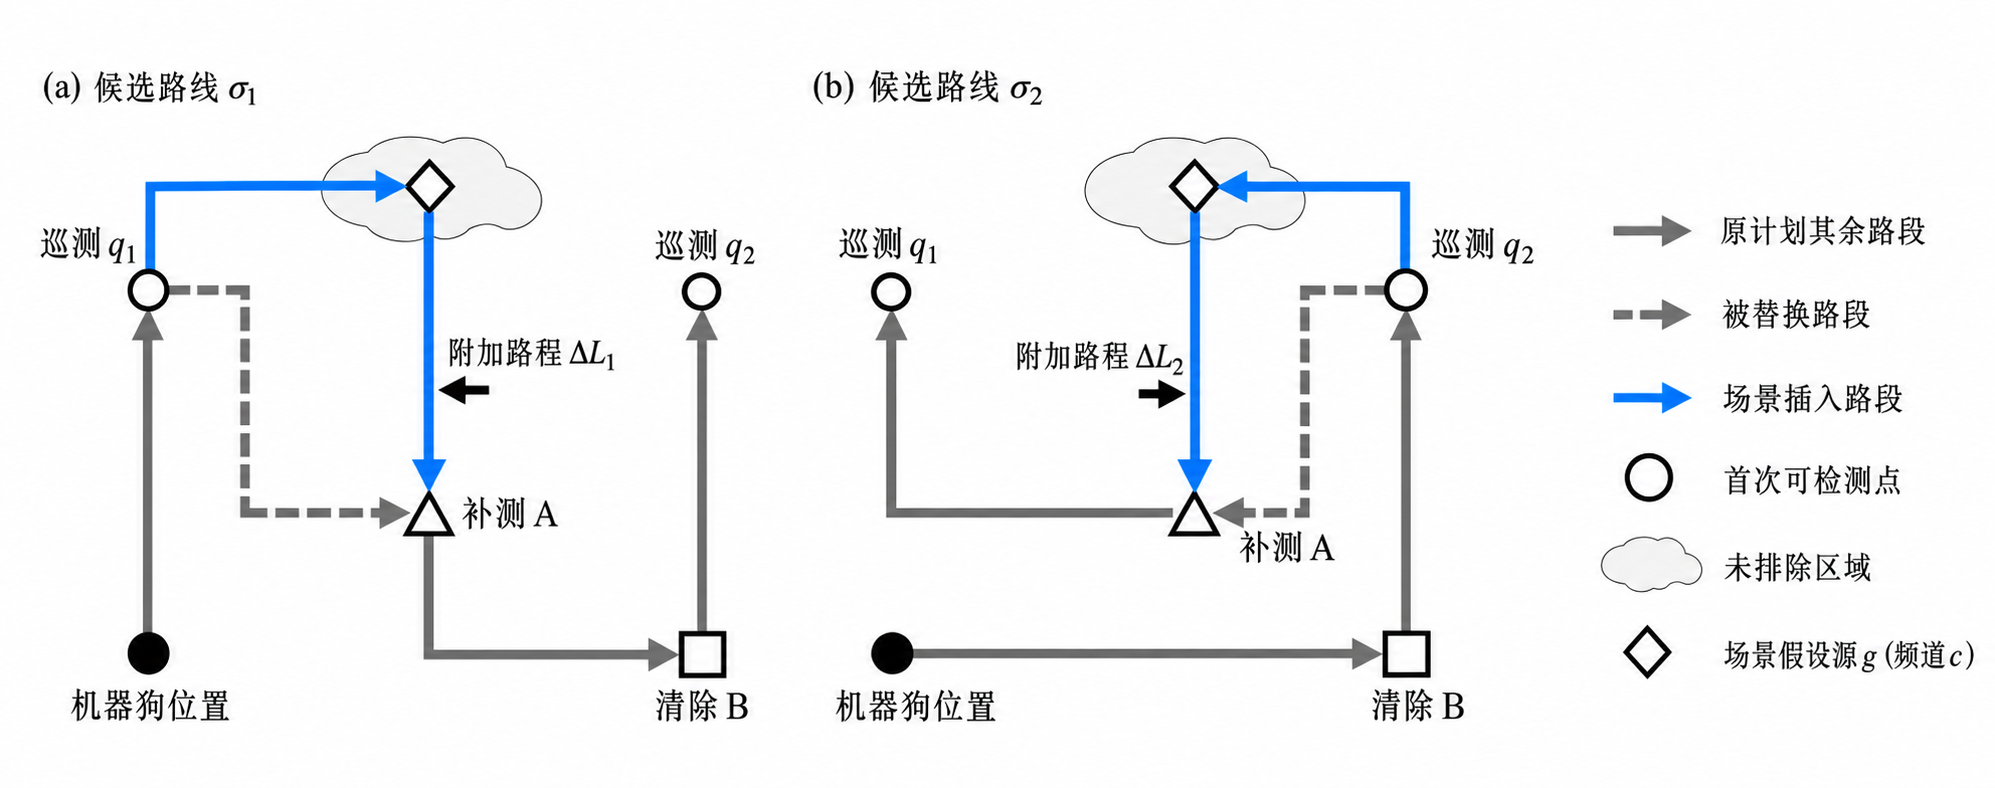
\includegraphics[width=\linewidth]{figures/q3_conditional_route_evaluation_paper.png}
\caption{条件场景下候选路线的附加代价估计}\label{fig:q3-scenario-routes}
\end{figure}

两条路线分别先在\(q_1\)、\(q_2\)检测到该假设源，因此在代价估计中用蓝色路段\(q_i\to g\to A\)替换灰色虚线路段\(q_i\to A\)。图中\(\Delta L_i\)为两段蓝线路程之和减去被替换路段的长度。发现频道\(c\)后，后续巡测点跳过该频道；将这一检测次数变化与附加移动计入式（33），再按式（34）对同批场景取平均，即得到候选路线的比较依据。

\subsubsection{滚动求解步骤}

\textbf{Step 1　初始化状态。} 令 \(p_0=(0,0)\)、\(\kappa_0=1\)、\(\mathcal D_0=\varnothing\)、\(\mathcal N_0=\mathcal C\)，并对所有频道取 \(H^-_{c,0}=\varnothing\)、\(U_{c,0}=\Omega\)。

\textbf{Step 2　生成未知频道检测行动。} 根据各频道当前的 \(U_{c,t}\) 生成满足式（26）的检测位置，并明确每个位置对应的检测频道，得到 \(\mathcal A_t^{\mathrm{scan}}\)。计算时采用可细分方格保守表示 \(U_{c,t}\)，仅当方格被排除圆完整覆盖时才删除，使有限采样点的覆盖判定对应连续区域的排除。

\textbf{Step 3　生成补充检测与清除行动。} 对每个 \(c\in\mathcal D_t\)，当 \(\mathcal G_{c,t}=\varnothing\) 时，根据当前定位区域生成补充检测行动；当 \(\mathcal G_{c,t}\ne\varnothing\) 时，按式（25）生成保证清除行动。二者分别组成 \(\mathcal A_t^{\mathrm{loc}}\) 与 \(\mathcal A_t^{\mathrm{clr}}\)。

\textbf{Step 4　构造候选路线。} 将三类候选行动组成 \(\mathcal A_t\)，从当前位置出发生成若干开放路线，并利用多起点、任务重插入与两交换（2-opt）调整行动次序；所有调整均保持式（26）的完整覆盖要求。

\textbf{Step 5　评价并选择路线。} 根据式（32）抽取同一批条件场景，按式（33）计算各候选路线的平均代理代价，并由式（34）选出当前路线。

\textbf{Step 6　执行首个行动并更新状态。} 仅执行 \(\sigma_t^*\) 的第一个行动，根据真实反馈按式（22）---（23）完成状态转移，再重新生成候选行动与路线。

\textbf{Step 7　检查终止条件。} 当式（27）成立时，任务结束，并按式（29）记录完整任务时间；否则返回 Step 2 继续滚动求解。

\subsection{独立案例验证}

在开发案例上确定策略及参数后，我们使用另外1000个随机案例检验本文策略。全部案例均完成清除并正常退出，剩余源总数为0。本文算法的平均每源耗时为212.77秒/源。

图\ref{fig:old4}给出逐例按源数归一化后的耗时分布与构成。95\%的案例每源完整退出耗时不超过269.92秒；失败清除的平均每源耗时仅为0.39秒。本文策略在1000个独立案例中实现了100\%的全清与正常退出率，失败清除的直接耗时占比仅为0.18\%，展现了可靠的任务完成能力与极低的无效清除直接开销。

\begin{figure}[H]
\centering
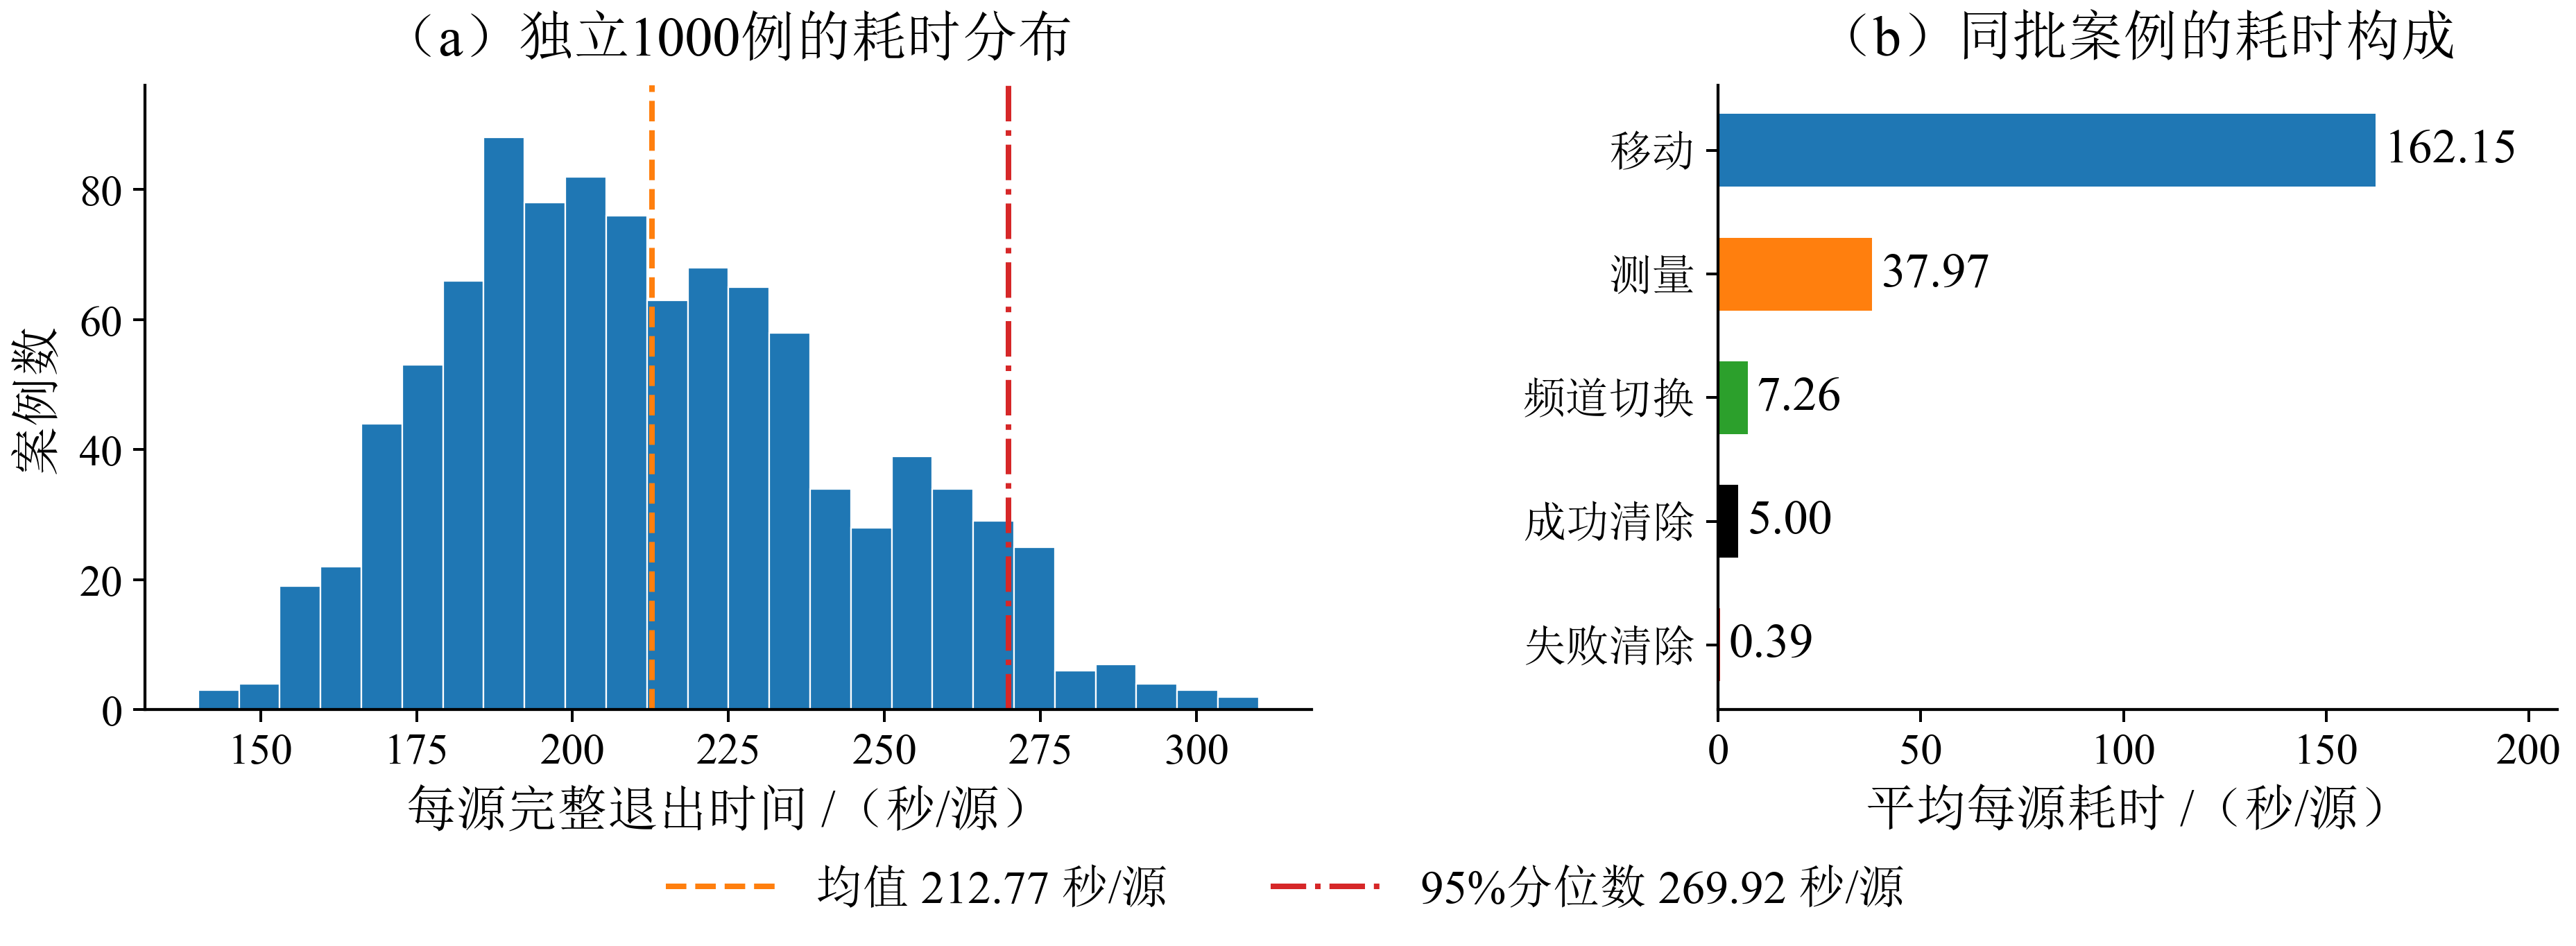
\includegraphics[width=0.96\linewidth,height=0.68\textheight,keepaspectratio]{figures/q3_time_distribution.png}
\caption{独立案例的每源耗时分布与耗时构成}\label{fig:old4}
\end{figure}

\subsection{正式测试结果}

我们在模拟器中完成第三问的三次正式测试，均清除了全部干扰源，结果见表\ref{tab:old7}。平均定位清除时间为该例完整退出虚拟耗时与清除源数的比值，程序运行时间为模拟器记录的现实执行时长。

\begingroup
\small
\setlength{\tabcolsep}{4pt}
\setlength{\TableInnerWidth}{\dimexpr\linewidth-6\tabcolsep\relax}
\renewcommand{\arraystretch}{1.22}
\begin{longtable}{@{}>{\centering\arraybackslash}p{0.390\TableInnerWidth}>{\centering\arraybackslash}p{0.170\TableInnerWidth}>{\centering\arraybackslash}p{0.260\TableInnerWidth}>{\centering\arraybackslash}p{0.180\TableInnerWidth}@{}}
\caption{问题3正式测试结果}\label{tab:old7}\\
\toprule
测试案例编码 & 清除干扰源个数 & 平均定位清除时间 /（秒/源） & 程序运行时间 / 秒 \\
\midrule
\endfirsthead
\multicolumn{4}{c}{表\thetable\quad 问题3正式测试结果（续）}\\
\toprule
测试案例编码 & 清除干扰源个数 & 平均定位清除时间 /（秒/源） & 程序运行时间 / 秒 \\
\midrule
\endhead
\midrule
\multicolumn{4}{r}{续下页}\\
\endfoot
\bottomrule
\endlastfoot
UJBC-A4W9-A6FZ-XYQF & 15 & 175.896 & 1.999 \\
CQFE-KMZK-43Z9-VC6H & 12 & 217.896 & 1.478 \\
5P3S-DMUG-M4NP-N8W4 & 10 & 247.627 & 1.771 \\
\end{longtable}
\endgroup

\Needspace{0.50\textheight}
\subsection{灵敏度分析与消融实验}

由100例开发集选定消融项后，我们在另100例上配对验证。各组均全清并正常退出，剩余源与失败案例均为0。消融时仅在仍有巡测站时优先巡测，其余规则不变。

\begingroup
\renewcommand{\baselinestretch}{1.05}\fontsize{10.5}{13}\selectfont
\setlength{\tabcolsep}{3.5pt}
\setlength{\TableInnerWidth}{\dimexpr\linewidth-6\tabcolsep\relax}
\setlength{\LTpre}{3pt}\setlength{\LTpost}{3pt}
\renewcommand{\arraystretch}{1.05}
\begin{longtable}{@{}>{\centering\arraybackslash}p{0.32\TableInnerWidth}>{\centering\arraybackslash}p{0.23\TableInnerWidth}>{\centering\arraybackslash}p{0.25\TableInnerWidth}>{\centering\arraybackslash}p{0.20\TableInnerWidth}@{}}
\caption{灵敏度与消融的100例配对验证结果}\label{tab:q3-analysis}\\
\toprule
设置 & 平均完整耗时 / 秒 & 平均每源耗时 /（秒/源） & 失败清除次数 \\
\midrule
\endfirsthead
\multicolumn{4}{c}{表\thetable\quad 灵敏度与消融的100例配对验证结果（续）}\\
\toprule
设置 & 平均完整耗时 / 秒 & 平均每源耗时 /（秒/源） & 失败清除次数 \\
\midrule
\endhead
\midrule
\multicolumn{4}{r}{续下页}\\
\endfoot
\bottomrule
\endlastfoot
完整算法（\(B=64\)） & 2756.47 & 215.96 & 162 \\
\(B=16\) & 2757.10 & 215.95 & 159 \\
\(B=32\) & 2758.49 & 216.00 & 165 \\
巡测优先（\(B=64\)） & 3736.31 & 292.66 & 132 \\
\end{longtable}
\endgroup

\begin{figure}[H]
\centering
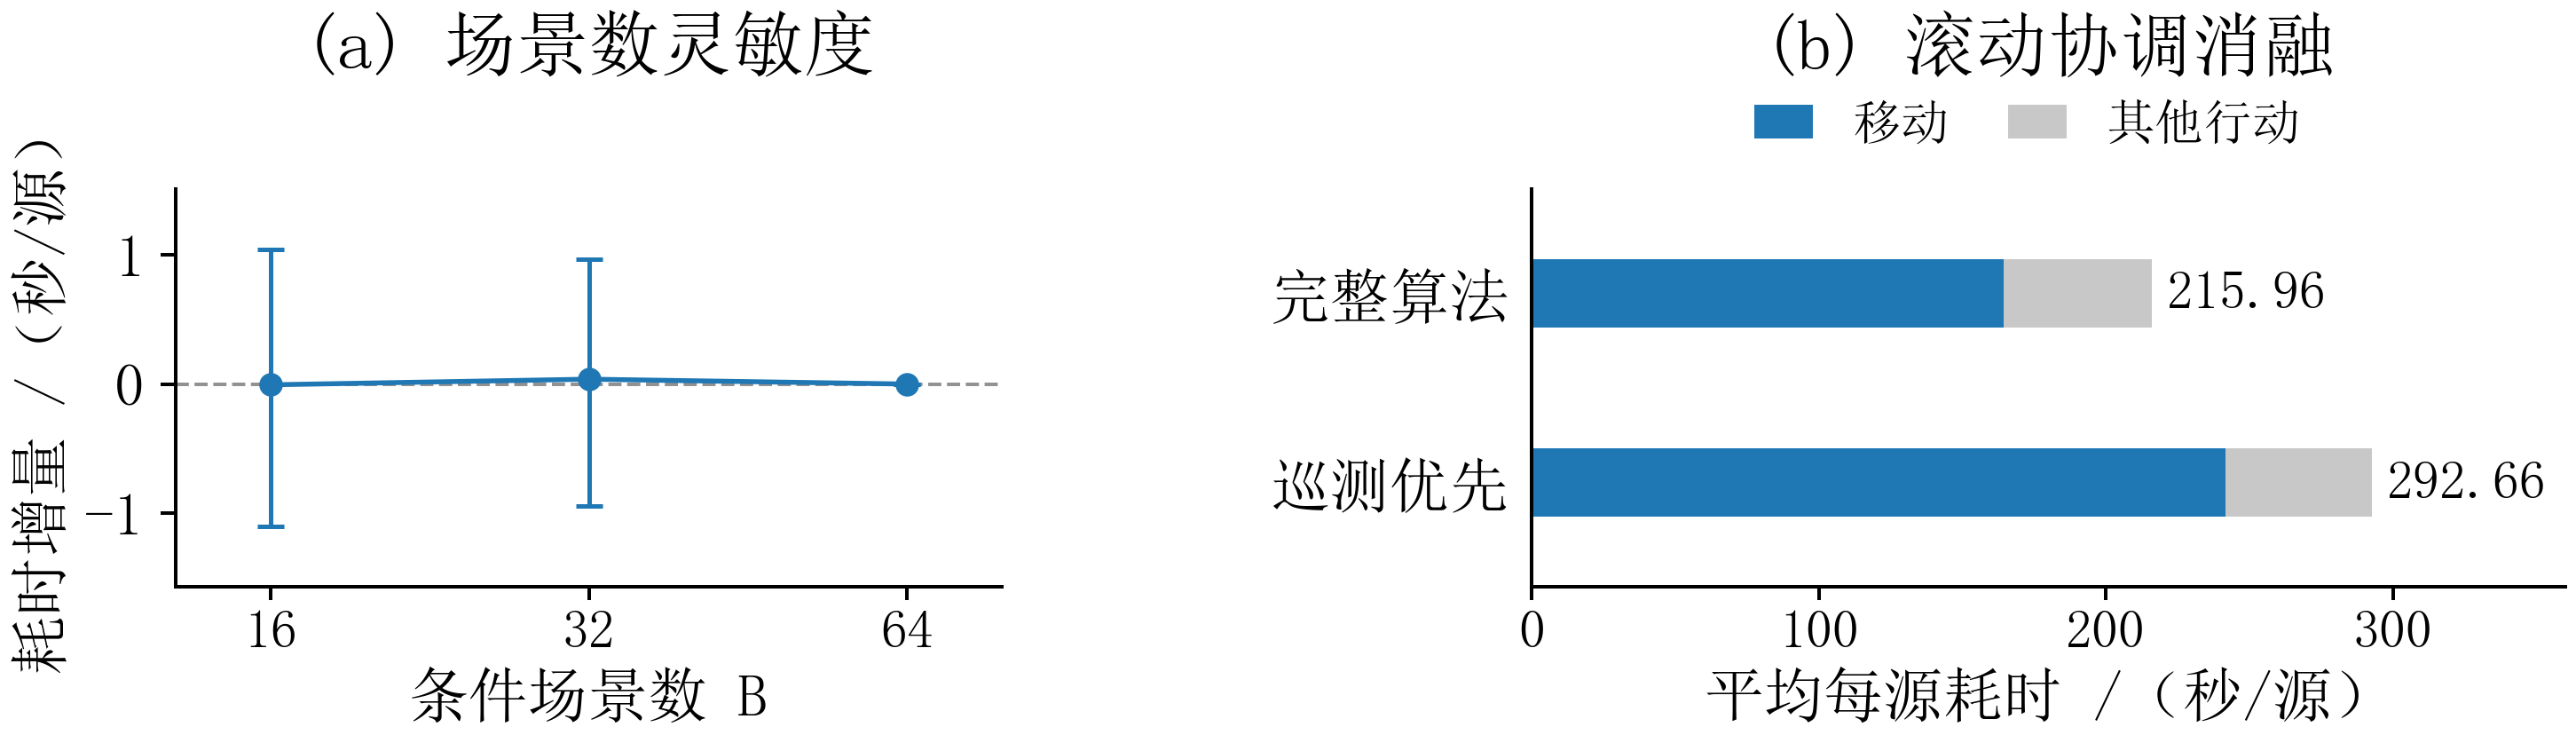
\includegraphics[width=\linewidth]{figures/q3_ablation_paired.png}
\caption{场景数灵敏度与滚动协调消融；左图以\(B=64\)为基准，误差棒为95\%配对区间}\label{fig:q3-analysis}
\end{figure}

灵敏度分析表明，算法的平均每源耗时在所测场景数范围内保持稳定，对该参数变化不敏感。消融实验表明，滚动协调通过减少移动开销，使平均每源耗时较巡测优先降低26.21\%。因此，在保证全部清除的前提下，穿插安排巡测与清除能够提高任务效率。
